\section{Estrategia de control de formaciones}
\setlength{\columnseprule}{0pt}
\onecolumn

Esta investigación enfrenta el problema de diseñar una ley de control $\mathbf{u}_i$ para cada agente $i \in \mathcal{S}$ que logre y preserve una formación deseada, evadiendo obstáculos en el proceso:
\begin{equation*}
    \lim_{t\to\infty} \|\mathbf{p}_i(t) - \mathbf{p}_i^\ast(t)\| = 0,
    \quad \forall\, i \in \mathcal{S}
\end{equation*}
\vspace{-1cm}
\begin{figure}[H]
    \centering
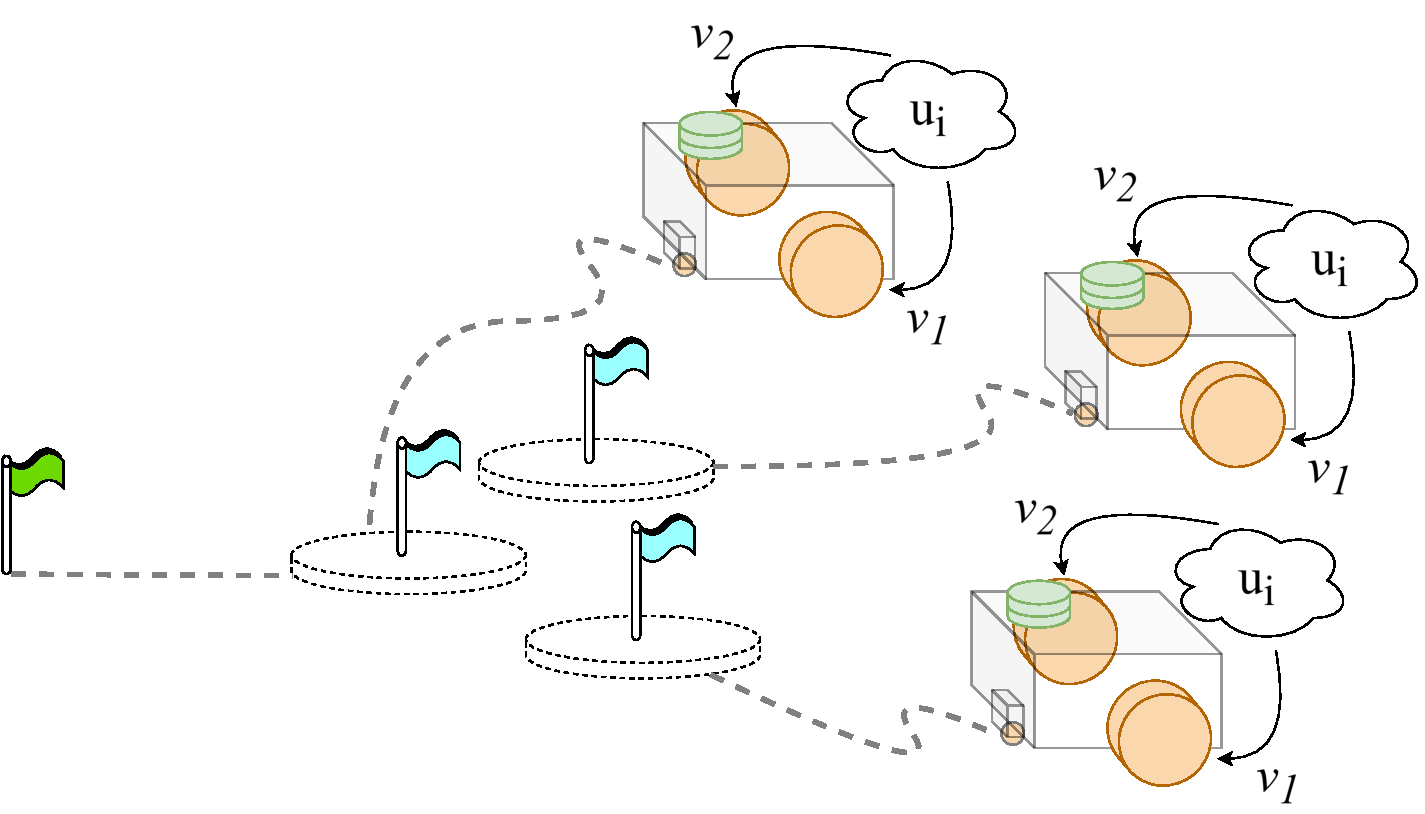
\includegraphics[width=0.4\linewidth]{Pics/extension.pdf}
    \caption{Flota de robots convergiendo a formación}
    \label{fig:extension}
\end{figure}